%\documentclass[a4paper,10pt]{book}
%\usepackage[utf8x]{inputenc}

\documentclass[12pt,letterpaper]{report}
%\usepackage{geometry,fancyhdr}

% \usepackage[spanish]{babel}
% \usepackage[utf8]{inputenc}

\usepackage{subfigure}
\usepackage{algorithm}
\usepackage{algorithmic}
\usepackage{listings}  
\usepackage{amsthm}
\usepackage{textcomp}
\usepackage{multicol}
\usepackage{float}
\usepackage{url}
\usepackage{enumerate}
\usepackage{newlfont}
\usepackage{psfrag}
\usepackage{charter}
\usepackage{setspace}
\usepackage{longtable}
\usepackage{subfigure}
\usepackage[dvips]{epsfig}
\usepackage[centertags]{amsmath}
\usepackage[size=normalsize]{caption}
\usepackage{newlfont}
\usepackage{psfrag}
\usepackage[utf8]{inputenc}
\usepackage[spanish]{babel}

%fonts matematicos
\usepackage{amsfonts}
\usepackage{amssymb}

\usepackage{framed}
% colocar un texto dentro de un cuadrado que lo contiene
%\begin{framed}
%\end{framed}

%\usepackage{tikz}

\usepackage{listings}
\usepackage{icomma}

%paquete necesario para incluir imaganes .eps en pdf
\usepackage{epstopdf}

\usepackage{UTFSM_Tesis}

\usepackage[active]{srcltx}
\usepackage[dvips, pdftitle={Jonathan Antognini memoria}, pdfauthor={Jonathan Antognini}, pdfsubject={Memoria}]{hyperref} 

%Modificar el formato de los capitulos, secciones y subsecciones, ademas modifica la visualizacion en la lista de contenidos.
  %\usepackage{titlesec}
  %\usepackage{titletoc}
 

\hfuzz2pt

\hypersetup{%
pdftitle={Memoria jantogni},
pdfauthor={Jonathan Antognini},
pdfkeywords={memoria, jantogni},
bookmarksnumbered,
pdfstartview={FitH},
urlcolor=cyan,
}%

\hyphenpenalty=5000
  \tolerance=1000
\hyphenation{no-me-cor-tes}


 \oddsidemargin  0cm    % Ancho Legal 21,59cm
 \evensidemargin 0.5cm  % Alto  Legal 35,56cm
 \textwidth      16.5cm
 \topmargin       -1.5cm
 %\voffset        2cm  % Margen superior
 \textheight     22cm
 %  \parindent      4cm
 %\parskip        2ex

\newlength{\defbaselineskip}
\setlength{\defbaselineskip}{\baselineskip}

\newcommand{\setlinespacing}[1]%
           {\setlength{\baselineskip}{#1 \defbaselineskip}}
% \newcommand{\doublespacing}{\setlength{\baselineskip}%
%                            {1.3 \defbaselineskip}}
% \newcommand{\singlespacing}{\setlength{\baselineskip}{\defbaselineskip}}

%Formulas matem?ticas utilizadas en el paper
\newcommand{\bbbr}{\mathbb R}

\newcounter{defcount}
\setcounter{defcount}{0}
\newenvironment{definition}[1]
%%\bf\normalsize
{% This is the begin code \bf
\stepcounter{defcount}{\noindent \bf \normalsize Definition \bf \arabic{defcount}: #1}\nopagebreak[3] \\
\begin{it}
}
{% This is the end code
\end{it}

}

\newcounter{defcount1}
\setcounter{defcount1}{0}
\newenvironment{property}[1]
%%\bf\normalsize
{% This is the begin code \bf
\stepcounter{defcount1}{\noindent \bf \normalsize Property \bf \arabic{defcount1}: #1}\nopagebreak[3] \\
\begin{it}
}
{% This is the end code
\end{it}
}





%Redefine plain page style
% \fancypagestyle{plain}{
% \fancyhf{}
% \renewcommand{\headrulewidth}{0pt}
% \fancyfoot[LE,RO]{\thepage}
% }
% 
% % Code for creating empty pages
% % No headers on empty pages before new chapter
% \makeatletter
% \def\cleardoublepage{\clearpage\if@twoside \ifodd\c@page\else
%     \hbox{}
%     \thispagestyle{plain}
%     \newpage|||
%     \if@twocolumn\hbox{}\newpage\fi\fi\fi}
% \makeatother \clearpage{\pagestyle{plain}\cleardoublepage}
% 
% % Define pagestyle
% \pagestyle{	fancy}
% \fancyhf{}
% \renewcommand{\chaptermark}[1]{\markboth{ \emph{#1}}{}}
% \fancyhead[LO]{}
% \fancyhead[RE]{\leftmark}
% \fancyfoot[LE,RO]{\thepage}


%U1 hasta olympiaCentrodecompras
% tomar micro 60 en el paradero del mall, 3 paraderos mas al norte, himmel.


\setlength\parindent{0pt}

\setcounter{secnumdepth}{5}
\setcounter{tocdepth}{5}

%The first line enables numbering of subsubsections. 
%The second line includes subsubsections in the table of contents.



\begin{document}

%\lstset{language=[ISO]C++}

\title{High frequency trading \& Graphics processing unit}
\author{Jonathan Andrés Antognini Cavieres}
\submitdate{Marzo - 2013}
\copyrightyear{2012}
%%%%%%%%%%%%%% Elegir uno de los siguientes grados:
%\ingej
\ingciv
%\phd

% \phd
%%%%%%%%%%%%%%
\profguia{Dr. Luis Salinas Carrasco}      % Cambiado a partir de supervisor
\profcorr{Dr. H\'ector Allende Olivares}         % Cambiado a partir de firstreader

%%%% dedicatorias al termino de la tesis %%%%
\dedicate{
 A mi familia
}

\nolistoffigures
\nolistoftables

\beforepreface


%  \listoftables	
%  \listoffigures
%  \listofalgorithms

%\input{agradecimientos.tex}

%%\begin{spacing}{.97}
\vspace*{2cm}
\thispagestyle{empty}
%\begin{center}
{\bfseries \Huge Abstract }
\vspace{1.5cm}

\begin{quotation}
The technical analysis of stock markets and foreign exchange market has been
used in order to forecast the behavior of the prices of a certain stock
or currency. Such analysis is based on the detection patterns of
a financial time series, which are known by its non-stationary and random
behavior.

%El análisis técnico de los mercados bursátiles y de divisas se ha utilizado
%para intentar predecir el comportamiento futuro de los precios de un activo o
%una divisa. Dicho análsis se basa en la detección de patrones en una serie
%temporal financiera, las que son conocidas por su comportamiento no
%estacionario y comportamiento aleatorio. 

An interest pattern to address is the integration and cointegration between the
prices of certain stocks or currencies, which establish that when two or more
time series are cointegrated, and considering that both processes are
non-stationary, such as as financial time series, there is a long term
equilibrium relation which link both series such that the relation is
stationary.  The model that take advantage of this scenario is the Vector Error
Correction (VECM)

%Un patrón de interés de estudio es la integración y cointegración entre los
%precios de ciertas divisas. Cuando dos o más series de tiempo están
%cointegradas, a pesar de que ambos procesos no sean estacionarios, como es el
%caso de las series de tiempo financieras, existe una relación de equilibrio a
%largo plazo que vincula ambas series tal que esta relación sea estacionaria. El
%modelo que permite aprovechar este partón es el Vector Error Correction Model
%(VECM).

The cointegration of pairs of currencies have been modeled in several studies,
particularly with FOREX data, which through software tools such as Matlab,
Eviews, etc.  it is possible to computationally forecast the behavior of those
time series.

%Existen varios trabajos donde modelan este problema con pares de monedas,
%particularmente con las series de tiempo del Foreign Exchange Market (FOREX).
%Además mediante herramientas computacionales como matlab, eviews, etc. es
%posible predecir computacionalmente el comportamiento de dichas series de
%tiempo.

However, an important aspect of this kind of series are their online nature,
since every second more information is generated due the Ask or Bid prices,
topic which hasn't been addressed completely.  VECM is a matricial model which,
if it is used in an online context, matrix updates are required to forecast.
%which implies the solution of a matricial system equation, to be able to
%forecast.

%Sin embargo un foco importante de este tipo de series es su caracter
%\emph{Online}, ya que a cada segundo se genera nueva información en el sistema
%debido a la compra o venta de divisas. Tema que no ha sido abordado
%completamente en la literatura. VECM es un modelo matricial, que desde el punto
%de vista \emph{Online}, sufre ciertas actualizaciones de valores, y para poder
%predecir es necesario resolver un sistema matricial.

On this work, we present the VEC, Sliding Windows VEC and Online VEC Models.
The objective of the Online VECM is to optimize the computational calculations,
reducing the number of times that the cointegration vectors are calculated.
Additionally, a class diagram and their implementation associated to Use Cases
was developed, considering: data reading, data re-sample in certain frequency,
graphics, metrics, etc. Additionally, we developed a couple of CUDA routines,
in order to optimize the calculation.

%En este trabajo se presenta el modelo VEC, el modelo VEC para ventanas
%deslizantes y la implementación \emph{Online} que busca optimizar cálculos
%computacionales reduciendo la cantidad de veces que se calculan los vectores de
%cointegración. Para ello se creo un diagrama de clases asociado a los casos de
%uso del modelo, considerando entre ello: lectura de datos, resample a cierta
%frecuencia, gráficos de resultados, etc.

I present the result of a set of tests with different currencies, ensuring all
the conditions to apply this model. The results shows that the Online VEC Model
version, reduce almost 50\% the execution time, maintaining the algorithm
accuracy. 

%Se realizaron pruebas con diferentes monedas de FOREX asegurando las
%condiciones para poder aplicar el modelo. Los resultados muestran que la
%versión \emph{Online} del modelo VEC, disminuye cerca del 50\% el tiempo de
%ejecución sin comprometer la precisión del algoritmo. Además se implementaron
%rutinas en CUDA para optimizar los tiempos de ejecución.

{\bf Keywords:} VECM, VAR, FOREX, GPU.
\end{quotation}

\newpage
% Español

\vspace*{2cm}
\thispagestyle{empty}
%\begin{center}
{\bfseries \Huge Resumen }
\vspace{1.5cm}

\begin{quotation}
El análisis técnico de los mercados bursátiles y de divisas ha sido utilizado
para intentar predecir el comportamiento de los precios de un activo o una
divisa. Dicho análsis se basa en la detección de patrones en una serie temporal
financiera, las que son conocidas por su comportamiento no estacionario y
aleatorio. 


Un patrón de interés de estudio es la integración y cointegración entre los
precios de ciertas divisas, el cual establece que cuando dos o más series de
tiempo están cointegradas, y considerando que ambos procesos no sean
estacionarios (como es el caso de las series de tiempo financieras), existe una
relación de equilibrio a largo plazo, que vincula ambas series para que esta
relación sea estacionaria. El modelo que permite aprovechar este partón es el
Vector Error Correction Model (VECM).

Existen varios trabajos donde modelan este problema con pares de monedas,
particularmente con las series de tiempo del Foreign Exchange Market (FOREX),
las cuales mediante herramientas computacionales como Matlab, Eviews, entre
otros, es posible predecir computacionalmente el comportamiento de dichas
series de tiempo.

Sin embargo un foco importante de este tipo de series es su carácter
\emph{Online}, ya que a cada segundo se genera nueva información en el sistema
debido a la compra o venta de divisas, el cual no ha sido abordado
completamente en la literatura.  VECM es un modelo matricial, que desde el
punto de vista \emph{Online}, sufre ciertas actualizaciones de valores, lo que
implica que para poder realizar una predicción es necesario resolver un sistema
matricial.

En este trabajo se presenta el modelo VEC, el modelo VEC para ventanas
deslizantes y la implementación \emph{Online} que busca optimizar cálculos
computacionales, reduciendo la cantidad de cálculo de los vectores de
cointegración.  Complementariamente, se creó un diagrama de clases asociado a
los casos de uso del modelo, considerando entre ello: lectura de datos,
resampleo a cierta frecuencia, gráficos de resultados, etc.

Se realizaron pruebas con diferentes monedas de FOREX, asegurando las
condiciones necesarias para poder aplicar el modelo. Los resultados muestran
que la versión \emph{Online} del modelo VEC, disminuye cerca del 50\% el tiempo
de ejecución sin comprometer la precisión del algoritmo. Adicionalmente, se
implementaron rutinas utilizando CUDA para optimizar el cálculo.

{\bf Palabras claves:} VECM, VAR, FOREX, GPU.

\end{quotation}


\afterpreface

\onehalfspacing

%\input{capitulo_1.tex}
%\input{capitulo_2.tex}
%\input{capitulo_3.tex}

\chapter{Introducción}
	\parindent=1.5em

A través de los años el hombre ha presentado un cambio sustancial en su nivel de vida; los conocimientos que ha logrado acumular y aplicar han sido para su beneficio,
y han cambiado radicalmente su modo de vivir. Existe una notable diferencia entre el hombre de hace unas cuantas décadas y el hombre moderno. Tal diferencia se ha
dado por el desarrollo de la ciencia, que está estrechamente relacionada con la innovación tecnológica. Por esta razón se amplía el contenido de cómo ha
evolucionado la ciencia y la tecnología en el mundo, su origen remoto, los países que más han aportado en esta área y su respectiva utilización, ya sea para
el desarrollo o la destrucción. Como se sabe, la tecnología se está haciendo presente en todas y cada una de las áreas de investigación, como física, química, 
biología, computación, y lo que es de interés para este documento es el área de los mercados financieros \cite{watsham1997quantitative}.

Esta memoria está enfocada a abordar un problema relacionado con las series financieras de alta frecuencia y una forma particular de poder realizar pronósticos tomando 
en cuenta las distintas características de naturaleza propia de este tipo de datos. Se pretende abordar esta problemática con metodologías computacionales, 
aplicando algunos análisis matemáticos útiles para esta área. El problema es de carácter financiero, por lo que es necesario contextualizar el tema mediante 
conceptos, criterios y términos generales asociados al área.

Este capítulo tiene como objetivo introducir los conceptos de series de tiempo financieras, sus orígenes y la alta frecuencia.

\section{Mercados Financieros}

El mercado financiero es un espacio con marco institucional que permite poner en contacto a oferentes y demandantes para que efectúen
transacciones financieras. La idea de mercado como foro organizado a la que acuden agentes económicos para efectuar transacciones
queda reducida en el mundo financiero como las bolsas de valores \cite{mishkin2006financial}.

El concepto de mercado financiero se utiliza en general para referirse a cualquier mercado organizado en el que se negocien instrumentos financieros
de todo tipo, como acciones, divisas, etc. El espacio para generar estas interacciones no necesariamente debe ser físico. Por otro lado, el negociar
instrumentos financieros implica a grandes rasgos: definir su precio e intercambiarlos, por ende, estos mercados están basados en
las fuerzas de oferta y demanda, ubicando a todos los oferentes en el mismo lugar, y así facilitarle la búsqueda a los demandantes. Dentro
de este tipo de mercado se distinguieron bloques de estudio en la economía moderna \cite{jensen1984theory}.

Una de las razones que hace importante este tipo de mercado, es su funcionalidad, ya que permiten: por un lado aumentar el capital, siendo esto uno 
de los casos favorables, ya que también hay probabilidades considerables de disminuir el capital; comercio internacional, como en los mercados de 
divisas, por ejemplo Forex; y reunir a quienes necesitan recursos financieros, con los que tienen recursos financieros. Factores que permiten generar los 
efectos de oferta y demanda.

En este tipo de mercado se definen los siguientes términos \cite{nevmyvaka2003electronic}:
\begin{itemize}
	\item \emph{Dealer}: Un dealer es un ente presente en los mercados que está dispuestos a comprar o vender.
	\item \emph{Orders}: Operación de compra/venta de activos.
	\item \emph{Bid price}: Precio al cual un \emph{dealer} está dispuesto a comprar.
	\item \emph{Ask price}: Precio al cual un \emph{dealer} está dispuesto a vender.
	\item \emph{Market orders}: instrucción del cliente al dealer, de comprar o vender al mejor precio posible dentro de los valores actuales del mercado.
		Esto asegura la realización de la transacción, pero no el precio.
	\item \emph{Limit orders}: es una orden para comprar a un valor máximo (precio determinado), o para vender a un valor mínimo (precio determinado).
		Esto le da al cliente el control sobre el precio al que se ejecuta el comercio, sin embargo, no garantiza la realización de la transacción.
\end{itemize}

El conjunto de \emph{Limit orders} forman los \emph{books} para cierto instrumento, los cuales proveen información detallada del mismo. Con estos datos
se forman los llamados bid-ask spreads, que es la diferencia entre el precios cotizados para una venta inmediata (oferta) y una compra inmediata (bid). 
También se generan los bid-ask qoute, el cual define cotas para el precio de transacción.

\subsection{Mercados bursátiles}
Los mercados bursátiles están clasificados dentro de los mercados de capitales, en donde se negocian activos financieros. Este tipo de mercado provee financiamiento
por medio de la emisión de acciones y permiten luego el intercambio de estas. La aplicación más directa de este tipo de mercados, son las bolsas de valores, cuyo
origen se remonta a finales del siglo XV en las ferias medievales de Europa. Las bolsas de valores se pueden definir como mercados organizados y especializados, en 
los que se pueden realizar transacciones de títulos de valores por medio de intermediarios autorizados. Estas bolsas ofrecen al público y a sus miembros facilidades, 
mecanismos e instrumentos técnicos que facilitan la negociación de títulos de valores susceptibles de ofertas públicas, y precios determinados mediante subasta \cite{levine1998stock}.

La principal función de las Bolsas de Valores es proporcionar a los participantes información objetiva, completa y permanente de los valores
y las empresas inscritas en la bolsa, sus emisiones y las operaciones que en ella se realicen. Además debeb supervisar las actividades. Las componentes de este 
sistema son los activos y las instituciones financieras, cuya misión es contactar demandantes y oferentes en los mercados donde se negocian los diferentes instrumentos 
o activos financieros. En el documento se hablará de instrumento, ya que pueden ser acciones, divisas, etc. los cuales quedan generalizados bajo ese concepto.

Dentro de los estudios de la economía, se habla de que este tipo de mercado es de competencia perfecta, ya que posee características
como: elevado número de compradores y vendedores; La decisión individual de cada uno de ellos ejercerá escasa influencia sobre el mercado global; 
Homogeneidad de los productos, es decir, no existen diferencias entre productos que venden los oferentes; Transparencia del mercado, todos los 
participantes tienen pleno conocimiento de las condiciones generales en que opera el mercado; Libertad de entrada y salida de empresas, todos 
los participantes, cuando lo deseen, podrán entrar o salir del mercado a costos nulos o casi nulos \cite{mankiw2011principles}. 

Sin embargo, Eugene Fama propuso la Hipótesis de eficiencia de los mercados \cite{malkiel2012efficient}, la cual dice que los mercados son eficientes cuando
son capaces de trasladar a los precios de los instrumentos financieros, todos los datos relevantes, por lo tanto, el precio refleja \emph{toda} la 
información disponible, y lo hace de manera insesgada. Cuando se cumplen estas condiciones, el precio del instrumento financiero se comporta como un 
\emph{Random Walk} \cite{fama1965random}, por lo que los resultados no pueden ser predichos sistemáticamente.

%Sin embargo, han existido varios estudios asociados a la Hipótesis del Mercado Eficiente, la cual dice que cuando los mercados financieros son eficientes, 
%son capaces de trasladar a los precios de los activos, en cualquier momento, todos los datos relevantes de esos activos, es decir, que el precio de esos activos 
%refleja en todo momento toda la información disponible sobre todos los valores y lo hace de manera insesgada. Este término lo propuso Eugene Fama en el año
%1970, para y se refirió a los procesos aleatorios que se comportan como juegos justos, cuyos resultados no pueden ser predichos sistemáticamente.

\section{Series de tiempo financiera}

La mayoría de los fenómenos que se estudian temporalmente, deben tomar en cuenta la dinámica de los proceso con la finalidad tener una 
comprensión general del proceso. Una herramienta útil en dicho objetivo es el análisis de series de tiempo. Una serie de tiempo, es una secuencia de datos, 
medidos en determinado momento de tiempo y ordenados cronológicamente, con esto se genera una secuencia de datos indexados por su marca temporal. Se pueden presentar 
casos de series de tiempo en una multitud de disciplinas como ingeniería, sociología, economía, finanzas por solo mencionar algunas de ellas.

El propósito fundamental es mostrar las técnicas que permitan hacer inferencias del proceso en estudio incluyendo su predicción. Esto se logra estableciendo modelos
probabilísticos hipotéticos que representen a los datos; y en consecuencia, se lleva a cabo el proceso de ajuste, que incluye desde la estimación hasta la 
predicción, una vez que se ha determinado un modelo satisfactorio para la muestra de datos. Los modelos de series deben considerar la naturaleza del fenómeno y 
determinar los factores que pueden ser incluidos en el.

En particular, el análsis de una serie de tiempo financiera puede enfocarse en estudiar de forma teórica y práctica la valoración de cierto instrumento en el tiempo,
como también los volúmenes transados, etc. Lo que se intenta es modelar la incertidumbre generada por las características propias de este fenómeno \cite{tsay2005analysis}. 

%En particular, el análisis de una series de tiempo financiera se refiere a la teoría y práctica de la valoración de instrumentos en el tiempo, 
%intentando modelar la incertidumbre generada por las características propias del fenómeno. Tanto la teoría económica 
%y sus series temporales contienen un elemento de incertidumbre \cite{tsay2005analysis}. 

Las características diferenciadoras han propiciado numerosos trabajos en las áreas de econometría y economía financiera desde los años 60. Por ello, en el área 
financiera las evidencias sobre patrones ha conducido a la formulación de distintos modelos matemáticos.
%financiera las evidencias sobre estructuras ha conducido a la formulación de distintos modelos matemáticos que se estudiarán en esta memoria.

\subsection{Descripción de serie financiera}

Una tendencia en el estudio de las series financieras, es el estudio del precio de un instrumento en el tiempo.
%Las series de tiempo financieras, se basan en el estudio del precio de un instrumento financiero en el tiempo. 
Existen varios tipos de precios que se pueden analizar, por un lado están los indicadores que se utilizaron en los primeros estudios formales, los cuales 
mostraban información al respecto de los precios de: \emph{apertura}, \emph{cierre}, \emph{el más bajo}, \emph{el más alto}, \emph{promedio}. Esos datos 
estaban orientados a tomar métricas respecto a la frecuencia \emph{día}. Una muestra gráfica de esta información sería la siguiente:
%con estos datos quedaban gráficos como el siguiente:

\begin{center}
	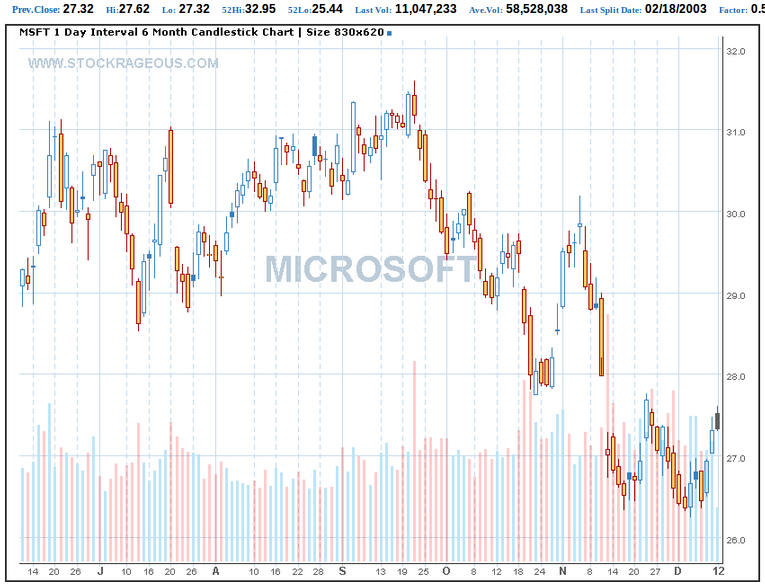
\includegraphics[width=0.8\textwidth]{images/microsoft} \\
	\textbf{Figura 1.} Información de los precios de microsoft en la bolsa. Tomada desde \url{http://www.stockrageous.com/}.
\end{center}

%Esos precios son a nivel diario, ya que los estudios en esos tiempos estaban orientados a esa frecuencia, como los flujos de caja, o análisis gráficos.
Por el tipo de frecuencia considerada en los datos, los estudios realizados estaban orientados a flujos de cajas o análisis gráficos. Sin embargo la data estudiada 
actualmente corresponde a data \emph{intra diaria}, la cual reside en los valores específicos en que se compró o vendió algún instrumento. 
Ese precio se conoce como el \emph{last price}, y corresponde al valor específico con el cual se realizó la transacción. La forma de como se efecúa este evento es 
mediante los \emph{market} o \emph{limit orders}, donde existe una cola de compras o ventas obtenidas mediante los \emph{limit orders} y que cuando se cumpla la 
condición asociada (de vender o comprar a cierto precio), se realiza la transacción y se registra dicho \emph{last price}; 
por otro lado, si se entra a comprar/vender directamente mediante una \emph{market order} también se registra dicho valor. Recopilando esa información, 
se puede generar una secuencia temporal de los \emph{last prices}. Estudios prácticos de estas series generalizan su gráfica con forma de \emph{U},
\cite{biais2012empirical}. 

%Por lo tanto, tomando en cuenta la alta frecuencia de estos datos, se torna muy complicado manejarlo de forma humana, es por esta 
%razón que es necesario realizar análisis cuantitativos usando computadores.

A través de la historia, estas interacciones se realizaban personalmente en las bolsas de comercio, en los llamados \emph{floor market} \cite{jain2005financial},
sin embargo con el avance de las tecnologías, se han implementado distintas plataformas de \emph{trading electrónico}: un método de negociación de instrumentos 
financieros por medios electrónicos \cite{weston2002electronic}. Estas tecnologías se utilizan para reunir a compradores y vendedores a través de plataformas de comercio 
electrónico, como por ejemplo: National Association of Securities Dealers Automated Quotation (NASDAQ), New York Stock Exchange (NYSE), etc. Tomando en cuenta las nuevas 
frecuencias de aparición de datos, en el orden de fracción de segundos, se torna difícil manejar los datos de forma humana, es por esta razón que es necesario realizar análisis 
cuantitativos mediante algoritmos computacionales.

Las series financieras de alta frecuencia tienen características singulares en relación a otras series, como son: 
\begin{itemize}
	\item Frecuencia: la frecuencia en la observación de los datos es mayor que en otro tipo de series de tiempo.
	\item Heterocedasticidad: ocurre cuando la varianza de las perturbaciones no es constante a lo largo de las observaciones.
		Este factor hace inadecuados los modelos desarrollados para series estacionarias.
	\item No estacionalidad: en muchos casos la media y varianza se presentan como no estacionarias.
	\item Información oculta: se pueden encontrar distintos tipos de patrones a diferentes niveles de escala.
\end{itemize}

\subsection{High frequency trading}

Con el paso del tiempo y la implementación de distintos sistemas de trading electrónico, la frecuencia de la data aumentó, pasando de minutos a fracciones de segundos. 
En estos sistemas se define un \emph{Tick}, como unidad atómica de información, particularmente sobre un instrumento determinado.
Esta unidad especifica una gran cantidad de parámetros como la marca temporal, precio, cantidad transada, etc. Los datos de alta frecuencia son un conjunto de datos 
de reportes detallados sobre la actividad y movimiento efectuados sobre un instrumento. Se reúne la información de los ticks con cierto intervalo de tiempo, 
el cual para este tipo de series es variable. El término utilizado para definir este fenómeno no es único \cite{ei2007quantitative}, existen distintos términos
para referirse a este tipo de datos, como (ultra-)high-frequency data, microstructure data, entre otros. 
%\emph{Wei Sun}, señala en \cite{ei2007quantitative} que en la literatura acuñan distintos términos para referirse a este tipo de datos.

Los sistemas informáticos que realizan la labor de facilitar el comercio de instrumentos financieros, son los llamados \emph{Electronic communication networks} (ECN).
Se crearon en 1998, año que fueron autorizados por la \emph{Securities and Exchange Commission}. La SEC es una organización estadounidense creada en 1933 \cite{hasbrouck2004economic}, 
y tiene la responsabilidad de velar por el cumplimiento de las leyes federales las bolsas de valores. Un caso emblemático, fue el 6 de mayo del 2010, fecha en la cual ocurrió el 
\emph{Flash-Crash} \cite{arndt2011high}, dio a lugar a una quiebra financiera estadounidense en el que el índice Dow Jones Industrial Average se desplomó un 9\%.

\section{High Performance Computing}

La capacidad de cómputo de los procesadores actuales ha incrementado, al igual que la cantidad de procesadores de las CPU y también las que tienen las tarjetas de video. Además, la
naturaleza de los problemas que se están estudiando, como simulación de tsunami, series de tiempo financiera, etc. generan una gran cantidad de cómputo, por lo que es
necesario optimizar y hacer más eficientes los algoritmos. Es por esto que nace el concepto de HPC, que es el área de desarrollo que aplica computadores de alto rendimiento 
(clusters) a tareas que implican alta cantidad de cómputo o requieren manejo de grandes volúmenes de información. 
%La idea base consiste en dividir los problemas en sub-problemas que se asignan a diferentes cores de un nodo o diferentes nodos de cálculo, coordinados por un nodo maestro mediante una red de alta velocidad. 

\subsection{Graphics Processing Unit}
%CUDA
Las siglas GPU provienen de Graphics Processing Unit, o en español Unidad de procesamiento gráfico. Para efectos de hardware, la GPU funciona como coprocesador,
pudiéndose utilizar de forma simultánea a la CPU y así aprovechar el potencial que puedan ofrecer ambas al mismo tiempo. Una GPU es un procesador
diseñado para llevar a cabo cálculos necesarios implicados en la generación de gráficos, ya sea, para un video juego, o como para una aplicación que utilice
gráficos en 2D, o 3D. Hoy en día las GPU son muy potentes y pueden incluso superar frecuencias de reloj de una CPU antigua.

Una GPU está formada por cientos de pequeños núcleos que trabajan juntos para procesar los datos de alguna aplicación. Esta arquitectura de procesamiento paralelo
masivo es la que proporciona al GPU su alta capacidad de cálculo. Existen numerosas aplicaciones aceleradas en la GPU que brindan una forma rápida de acceder
a la computación de alto desempeño (High Performance Computing). Durante los últimos años se han desarrollado nuevas tecnologías y arquitecturas
que permiten sacar mayor provecho a sus capacidades \cite{owens2007gpu}.

El concepto implícito en todo este tema es el paralelismo, que es una forma de computación en la cual varios cálculos pueden realizarse simultáneamente,
siempre y cuando no existan dependencias secuenciales entre ellos. Basándose en "divide y vencerás", principio que busca dividir los problemas grandes, para
obtener varios problemas pequeños, que son posteriormente solucionados en paralelo.

La evolución de las tarjetas gráficas ha venido acompañado de un gran crecimiento en el mundo de los videojuegos y las aplicaciones 3D, realizándose grandes
producciones de chips gráficos por parte de grandes fabricantes, como NVIDIA, AMD (ex ATI). Los recientes desarrollos sobre GPU abarcan distintas áreas de la ciencia \cite{kirk2010programming},
como problemas astrofísicos (n-body simulation), modelamiento molecular, computación financiera, etc. En los últimos años también han aparecido 
conjuntos de herramientas y compiladores que facilitan la programación de las GPUs, como por ejemplo, NVIDIA CUDA, que cuenta con la comunidad más activa hasta 
la fecha en programación de GPUs.

%\subsection{NVIDIA CUDA}
%Las primeras GPU fueron diseñadas como aceleradoras de gráficos y admitían apenas procesos específicos de funcionamiento fijo. En las últimas dos décadas,
%el hardware cada vez se volvió más programable, lo que culminó con la primera GPU de NVIDIA en los años 1999. En poco tiempo que se desarrollara el concepto de GPU,
%investigadores empezaron a utilizar el rendimiento de estas tarjetas en cálculos con punto flotante.
%
%Los dilemas que vivieron en futuro los programadores, fue que la programación para GPU estaba lejos de ser fácil, hasta que investigadores de la universidad de
%Stanford se propusieron reimaginar la GPU como un coprocesador de flujos.
%
%Puesto que NVIDIA sabía que su hardware era bueno e iba creciendo muy rápido, debían combinarse con herramientas de hardware y software intuitivas, invitaron
%a un equipo de investigación y desarrollo, para empezar a evolucionar una solución que ejecutara el lenguaje de programación C a la perfección en el GPU.
%Al reunión software y hardware, NVDIA lanzó al mercado CUDA en el año 2006. La competencia AMD tuvieron intentos forzosos en generar algo similar, pero su comunidad
%de desarrollo no tuvo la misma motivación que si tuvo NVIDIA CUDA.
%
%CUDA es una plataforma de computación paralela y un modelo de programación creado por NVIDIA. La tecnología implementada por NVIDIA, es un entorno basado en el 
%lenguaje C, que permite a los programadores escribir software para resolver problemas computacionales complejos en menos tiempo aprovechando la gran capacidad 
%de procesamiento paralelo de las GPU multinúcleo. Miles de programadores están utilizando las herramientas gratuitas de desarrollo de CUDA (válidas para millones 
%de GPU que circulan en el mercado), a fin de acelerar todo tipo de aplicaciones, desde herramientas de codificación de audio y video, diseño de productos, 
%investigación científica, etc. \cite{kirk2007nvidia}.
%
%Actualmente NVIDIA ofrece un kit de herramientas de CUDA, las cuales incluyen un compilador, bibliotecas de matemáticas, herramientas para corregir y optimizar
%rendimiento de aplicaciones. Encontrándose también con muestras de código, guías de programación, manuales de usuario, referencias de la interfaz de programación
%de aplicaciones (API) y otra documentación para ayudar al usuario dar los primeros pasos en el área. Cabe destacar que ofrece todo esto de forma gratuita,
%incluyendo NVIDIA Parallel Nsight for Visual Studio, el primer entorno de desarrollo del sector para aplicaciones masivas paralela que usan tanto GPU como CPU, esto
%en sistemas operativos Windows.

\section{Motivación}

Las características que presentan las series financieras de alta frecuencia son un problema recurrente y el estudio en esta área se torna a veces complicado.
Uno de los enfoques de solución para este tipo de problema es realizar análisis mediante el uso de descomposición Wavelet Multi-escala \cite{benaouda2006wavelet}, y 
los resultados son alentadores. Este enfoque se ha utilizado en distintas áreas de la ciencia, y en particular en series financieras. Más en particular Zhang ha propuesto 
un modelo neural-wavelet \cite{zhang2001adaptive}, mezclando redes neuronales con wavelet multiescala, los cuales llegan a buenas aproximaciones pero no logran competir 
en eficiencia temporal. Este último modelo, no ha sido aplicado para este tipo de serie.

%Estas series en la literatura se trabajan como series de tiempo, lo cual es una secuencia de observaciones ordenadas mediante índices, los cuales
%son la marca temporal, información contenida en los \emph{tick}. 

Los \emph{\textbf{objetivos principales}} son:
\begin{itemize}
	\item Implementar un modelo de predicción Neural-Wavelet basado en el modelo de Zhang y analizar su comportamiento con series
		financieras de alta frecuencia.
	\item Optimizar dichos algoritmos usando computación heterogénea (CPU + GPU) para aumentar su rendimiento.
\end{itemize} 
%es implementar un modelo de predicción Neural-Wavelet basado en el modelo de Zhang,
%de alta frecuencia y aumentar su eficiencia optimizando algoritmos.

Los \emph{\textbf{objetivos secundarios}}:
\begin{itemize}
	\item Adaptar el modelo de Zhang para este tipo serie, encontrando los parámetros apropiados.
	\item Encontrar una combinación de carga para CPU y GPU que permita hacer más eficiente los cálculos.
\end{itemize}
%Como objetivo secundarios se busca: encontrar una combinación que permita hacer más eficiente los cálculos, combinando la GPU con la CPU. 

\section{Organización de la Memoria}

Esta memoria se organizará con el siguiente esquema:
\begin{itemize}
	\item Capítulo 2: Estado del arte: se estudiarán y repasarán las técnicas relativas a .
	\item Capítulo 3: Descripción formal del problema: se formalizará el problema a resolver, indicando las características consideradas.
	\item Capítulo 4: Solución propuesta: se definirá una propuesta de solución, con la respectiva metodología de implementación. 
	\item Capítulo 5: Estudio experimental: se implementará y testeará la solución propuesta, comparando sus resultados.
	\item Capítulo 6: Conclusiones: se realizarán conclusiones generales del trabajo realizado y se detallarán posibles trabajos futuros.
\end{itemize}


\chapter{Estado del arte}
	En este capítulo se estudiarán las aplicaciones y estudios hechos en el área. Para ordenar esta sección, se
realizarán divisiones respecto al tema de fondo de estudio (HFT), los métodos cuantitativos a usar (neural-wavelet)
y finalmente el medio que pretende optimizar el rendimiento (GPU).

\section{High Frequency Trading}

\section{Wavelet Multiscale}

\section{Artificial Neural Network}

\section{Graphics Processing Unit}


\chapter{Descripción del problema}
	\section{Descripción histórica}
\section{Descripción y formalización a usar}


\chapter{Solución propuesta}
	\section{Algoritmo y fundamentos teóricos}


\chapter{Estudio experimental}
	\section{Selección de data (sector, frecuencia)}
\section{Parámetros del algoritmo}
\section{Validación}
\section{Speed up: multicore, gpu, híbrido}


\chapter{Conclusiones}
	Lorem ipsum dolor sit amet, consectetur adipiscing elit. Aenean eget tellus
dignissim, porta leo id, placerat est. Nam a libero nec arcu hendrerit pharetra
at a mi. Donec sagittis quis est id tempor. Maecenas imperdiet, mi at
sollicitudin faucibus, tellus turpis auctor lorem, ac lacinia magna tortor sit
amet neque. Ut iaculis sit amet purus sed consequat. Nunc pretium est non erat
lacinia faucibus. Phasellus id rutrum mi. Morbi nunc nisi, mattis sit amet
purus eget, convallis tristique urna. Curabitur quis tellus placerat, eleifend
nisi eget, scelerisque quam. Nulla et sapien fermentum, dictum elit non,
elementum elit.

Morbi pretium dolor vel vestibulum pulvinar. Donec lobortis arcu malesuada
augue dictum, et pulvinar lectus viverra. Praesent rhoncus, sapien sed
porttitor volutpat, nisi ex mattis massa, tincidunt accumsan sapien sem et
elit. Maecenas sed sem accumsan, sollicitudin nunc quis, imperdiet lectus.
Maecenas ut arcu vitae odio suscipit sollicitudin. Pellentesque sed est lacus.
Quisque nec lorem sem. Nulla tristique tempus lacus, ornare maximus magna
interdum non. Proin aliquet quis ligula eget condimentum. Phasellus egestas in
libero posuere dapibus. Sed vestibulum ullamcorper arcu, eu tempus lacus
ultrices at. Ut id commodo erat, tincidunt suscipit mi. Donec suscipit lacus
sed ex molestie, nec dignissim nunc volutpat. Cras a mollis tortor, a egestas
enim. Vestibulum rhoncus orci eget purus volutpat, non viverra justo porttitor.

Ut a nulla tortor. Nam urna tortor, accumsan eu est a, rutrum ornare lectus.
Nam vestibulum libero sed consectetur vehicula. Sed non neque nec velit sodales
feugiat consequat eu tellus. Sed ut elit rutrum ipsum tristique tempus.
Phasellus sit amet porta dolor. Fusce sodales bibendum tellus vel ultrices.
Integer vitae laoreet eros.


\singlespacing
\bibliographystyle{alpha}
%\bibliographystyle{plain}
\nocite{*} %quitar para mostrar s?lo lar referencias citadas.
\bibliography{references}

\end{document}

